%% v3.4 [2023/09/12]
\documentclass[technicalreport]{ieicej}
\usepackage[dvipdfmx]{graphicx,xcolor}
\usepackage[fleqn]{amsmath}
\usepackage{amsthm}
\usepackage{newtxtext}
\usepackage[varg]{newtxmath}
\usepackage{placeins}
%\usepackage{amssymb}
\usepackage{url}\urlstyle{rm}
\newtheorem{definition}{定義}

\def\IEICEJcls{\texttt{ieicej.cls}}
\def\IEICEJver{3.4}
\newcommand{\AmSLaTeX}{%
 $\mathcal A$\lower.4ex\hbox{$\!\mathcal M\!$}$\mathcal S$-\LaTeX}
%\newcommand{\PS}{{\scshape Post\-Script}}
\def\BibTeX{{\rmfamily B\kern-.05em{\scshape i\kern-.025em b}\kern-.08em
 T\kern-.1667em\lower.7ex\hbox{E}\kern-.125em X}}

%\tecrepyear{2023}
\jtitle{木幅学習システムの構築}
\jsubtitle{高効率なグラフ解析に向けた木幅概念の学習システム構築}
\etitle{Development of a Learning System for Treewidth}
\esubtitle{Constructing a System for Acquiring the Concept of Treewidth for Highly Efficient Graph Analysis}
\authorlist{%
 \authorentry{小林 紹子}{Shoko Kobayashi}{Kanagawa}
 %\authorentry[hana_ko@denshi.ac.jp]{電子 花子}{Hanako DENSHI}{Tokyo}% xxx
 \authorentry{玉木 久夫}{Hisao TAMAKI}{Kanagawa2}% 
 \authorentry{井口 幸洋}{Yukihiro IGUCHI}{Kanagawa}% 
}
\affiliate[Kanagawa]{明治大学理工学部情報科学科\hskip1zw
  〒214--0033 神奈川県川崎市多摩区東三田1--1--1}
 {Dept.of Computer Science,
  Meiji University\hskip1em
  1--1--1 Higashimita, Tama-ku, Kawasaki-shi, Kanagawa,
  214--0033 Japan}
\affiliate[Kanagawa2]{明治大学 研究・知財戦略機構 \hskip1zw
  〒214--0033 神奈川県川崎市多摩区東三田1--1--1}
 {Organization for the Strategic Coordination of Research and Intellectual Properties,
  Meiji University\hskip1em
  1--1--1 Higashimita, Tama-ku, Kawasaki-shi, Kanagawa,
  214--0033 Japan}

  

%\MailAddress{$\dagger$hanako@denshi.ac.jp,
% $\dagger\dagger$\{taro,jiro\}@jouhou.co.jp}

\begin{document}
\begin{abstract}
木幅はグラフ理論やアルゴリズム設計において重要な概念であるが，
その抽象度の高さや日本語教材の不足により，初学者にとって理解が難しいという課題がある．
そこで本研究では，木幅および木分解の定義理解を促進することを目的とした
Webアプリケーションによる学習支援システムを構築した．
提案システムでは，グラフ構造や木分解を視覚的かつインタラクティブに操作でき，
問題演習を通じて段階的な理解を支援する．
実装には Node.js，Next.js，React，TypeScript，SQLite，Prisma，ReactFlow を用い，
学習コンテンツの作成・拡張が容易となるよう設計した．
\end{abstract}

\begin{keyword}
グラフ理論, 木幅, 木分解, Next.js, ReactFlow, React, TypeScript
\end{keyword}
\begin{eabstract}
Despite their significance in algorithm design, treewidth and tree decomposition are difficult to grasp due to their abstraction and a lack of Japanese resources. 
This paper presents a web-based learning system designed to facilitate a deeper understanding of these concepts. 
The platform offers a visual environment where users intuitively explore graph structures through interactive exercises. 
Built with modern web technologies and ReactFlow, the system enables dynamic graph manipulation and visualization. 
Furthermore, an administrative interface allows instructors to efficiently create and manage custom learning modules, streamlining the delivery of educational content.
%英文アブストラクト 100 words
\end{eabstract}
\begin{ekeyword}
graph theory, treewidth, tree decomposition, Next.js, ReactFlow, React, TypeScript
\end{ekeyword}
\maketitle

\section{はじめに}
グラフ理論\cite{wilson1979introduction}は，
ディペンダブルコンピューティング分野における信頼性解析や，
ソフトウェア分野におけるコンパイラのレジスタ割り当て，
スケジューリングなど，
多くの分野で基礎理論として重用されてきた．

一般に，解くことが困難な問題であっても，
対象となるグラフが木構造であれば容易に解けることが知られている．
木分解とは，一般グラフの頂点集合を部分集合（バッグ）に分割し，
それらを木構造で接続することで，一般グラフ上の問題を木構造上の問題として扱えるようにする.
また，木幅とはグラフがどの程度「木に近い構造を持つか」を表す指標であり，木分解を用いて求められる\cite{robertson1986graph}．
木幅が小さいグラフでは，
幅の小さい木分解が存在するため，
各バッグに含まれる頂点数が少ない構造で表現でき，
効率的なアルゴリズムを設計できることが知られている\cite{robertson1986graph}．
代表的な応用例として，
最大独立集合問題，グラフ彩色問題，最短経路問題などが挙げられる．

また，木幅が小さい場合，各バッグ内の状態数が限定されるため，
動的計画法を適用しやすいという利点がある．
このように木幅は多くの問題に対して有用な概念であるが，
その抽象性や木分解構築の難しさから理解のハードルが高く，
日本語で学べる教材や可視的に学習できる環境は十分とは言えない．
そこで本研究では，
木幅および木分解の定義理解を促進することを目的とした
学習システムを構築したので，
その内容について報告する．


\section{木幅（treewidth）とは}
本節では，グラフ理論の基本的な用語について概説する．
詳細は文献\cite{wilson1979introduction,robertson1986graph,diestel2025graph}を参照されたい. 

\subsection{木と閉路}
閉路とは，始点と終点が一致し，それ以外の頂点を重複せずに通る道である.
グラフ理論において，閉路の存在はグラフ構造の複雑さを特徴づける重要な要素の一つであり，多くの計算問題において困難性の原因となる.

一方，木とは，閉路を含まず，かつ連結である無向グラフである. 
木は極めて単純な構造を持つグラフであり，以下の性質が知られている\cite{wilson1979introduction}.
\begin{itemize}
  \item 木は閉路を含まない連結グラフ,
  \item 任意の二頂点間にただ一つの単純路が存在する,
  \item 任意の辺を一つ削除すると，グラフは非連結になる
\end{itemize}
図\ref{tree}に木と閉路のあるグラフを示す.

特に，任意の二頂点間に単純路が一意に定まるという性質は，木構造における情報の伝播や分割を容易にしている. 
さらに，木において葉（次数1の頂点）以外の任意の頂点を一つ削除すると，グラフは複数の連結成分に分割される.
この性質により，木は自然な再帰構造を持ち，分割統治法や動的計画法を適用しやすい対象となる.
\begin{figure}[h]
  \centering
  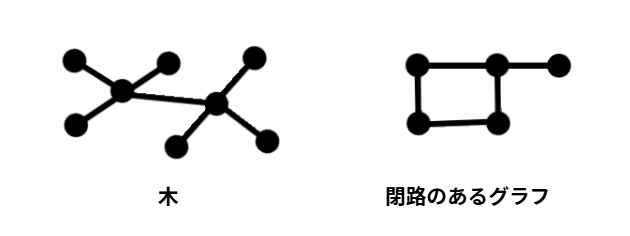
\includegraphics[width=0.5\textwidth]{tree.png}
  \caption{木と閉路のあるグラフ}
  \label{tree}
\end{figure}
\begin{figure}[h]
  \centering
  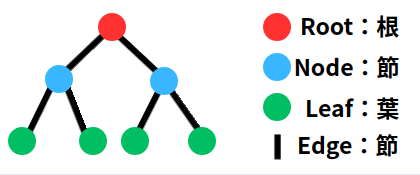
\includegraphics[width=0.4\textwidth]{tree_instruction.png}
  \caption{木構造の用語}
\end{figure}
このような構造的単純性のため，最大独立点問題など多くの計算困難な問題であっても，入力グラフが木である場合には多項式時間，あるいは線形時間で解くことが可能である．
一方で，一般のグラフは閉路を多く含み，木のような単純な構造を持たない場合が多い. 
そのため，任意の一般グラフに対して，直接木と同様のアルゴリズムを適用することは困難である. 

そこで，一般グラフを「完全な木」ではなく，「木に近い構造」として捉え，その上で計算を行う枠組みが考えられてきた. 
この考え方を形式化した概念の一つが\textbf{木分解（tree decomposition）}である.

\subsection{木分解（tree decomposition）}
\textbf{木分解（tree decomposition）}とは，一般のグラフの頂点集合を部分集合の集まりとして分割し，それらの関係を木構造で表現する手法である. 
これにより，元のグラフの構造的複雑さを，木構造上で扱うことが可能となる. 
木分解は，一般グラフ上の問題を木構造上の問題として扱うための基盤となる概念であり，これを測る指標として木幅が定義される.
木分解は以下のように定義される\cite{robertson1986graph}.

\begin{definition}
$V$をグラフ$G$の頂点集合, $E$を辺の集合とする.また, $I$を木$T$の頂点集合, $F$を辺の集合とする. 
グラフ $G = (V, E)$ の木分解とは，
木 $T = (I, F)$ と，各 $i \in I$ に対応する頂点集合$\{ X_i \mid i \in I \}$\it(bags（バッグ）と呼ばれる)からなる組$(\{X_i \mid i \in I\},\ T)$
であって，次の条件を満たすものをいう．

\item[(TD1)] 全ての頂点がどこかのバッグに含まれる.
  \[
    \bigcup_{i \in I} X_i = V
  \]

      
  
  \item[(TD2)] グラフGの辺を構成する頂点は必ず同じバッグに含まれる.
 \[
  \forall (u,w) \in E,\ \exists i \in I \text{ で } u \in X_i \text{ かつ } w \in X_i
\]
    

  \item[(TD3)] 同一頂点を含むバッグ$X$は木$T$ 上で連結である.
  \[
  \forall i,j,k \in I,\ 
  j \in \mathrm{path}_T(i,k)
  \Rightarrow
  X_i \cap X_k \subseteq X_j
\]
ここで$\mathrm{path}_T(i,k)$は, 木Tにおいて頂点$i$から頂点$k$を結ぶ唯一の単純路を意味する.    
  \end{definition}


\subsection{木幅（treewidth）}

木分解を用いることで，一般のグラフを木構造として扱うことが可能になるが，
その際に重要となるのが「どれだけ小さな部分集合で分解できるか」である．
直感的には，木分解における各バッグの大きさが小さいほど，
元のグラフは「木に近い構造」を持つと考えられる．

この考えを定量的に表した指標が\textbf{木幅（treewidth）}である．

\begin{definition}
木分解 $(\{X_i \mid i \in I\}, T)$ の幅とは，
\[
\max_{i \in I} (|X_i| - 1)
\]
で定義される値である．
\end{definition}

ここで，各 $X_i$ は木分解におけるバッグを表し，
その大きさ $|X_i|$ は同時に扱う必要のある頂点数を意味する．
定義において $-1$ を行うのは，
木に対して木幅が1となるように調整するためである．

次に，グラフ全体に対する木幅を定義する．

\begin{definition}
グラフ $G$ の\textbf{木幅（treewidth）}とは，
$G$ のすべての木分解の幅の最小値である．
\end{definition}

木幅はグラフの不変量であり，
グラフがどの程度「木に近い構造を持つか」を表す指標である．
木幅が小さいグラフほど，
木構造上で有効な分割統治法や動的計画法を適用しやすい．

また，木分解は部分木の集合として捉えることもできる．
木分解の定義における条件 (TD3) により，
ある頂点 $v \in V(G)$ を含むバッグの集合は
木 $T$ 上で連結な部分木 $T_v$ を形成する．
さらに，条件 (TD2) により，
辺 $uv \in E(G)$ に対しては
部分木 $T_u$ と $T_v$ が共通のバッグを持つことが保証される．

図3のグラフに対し,これらの条件を満たす木分解の一例を図4に示す.
頂点集合$X_i$において(TD1), (TD2)が満たされていることがわかる.
また, 図4の点線は, バッグ$X$が(TD3)を満たしてること示している.
木$T$の3節点を構成するバッグ$X_1, X_2, X_3$の要素はいずれも3である.
したがって，この木分解の幅は2であり，これ以外にも木分解は存在するが，2が最小なので図3のグラフの木幅は2である.

\begin{figure}[h]
  \centering
  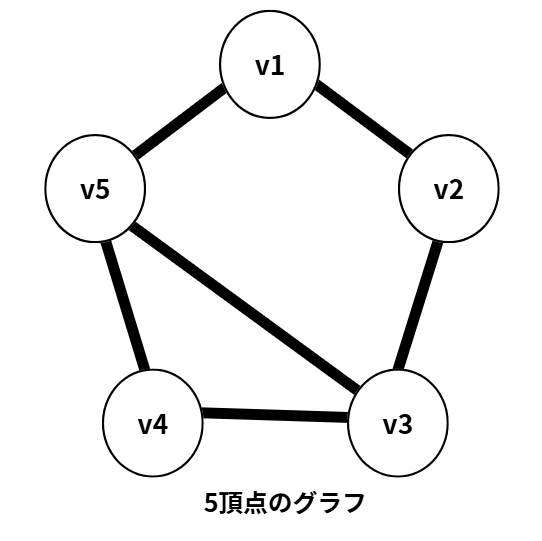
\includegraphics[width=0.3\textwidth]{5-nodes-tree-diagrams.png}
  \caption{5頂点のグラフの場合}
\end{figure}  
\begin{figure}[h]
  \centering
  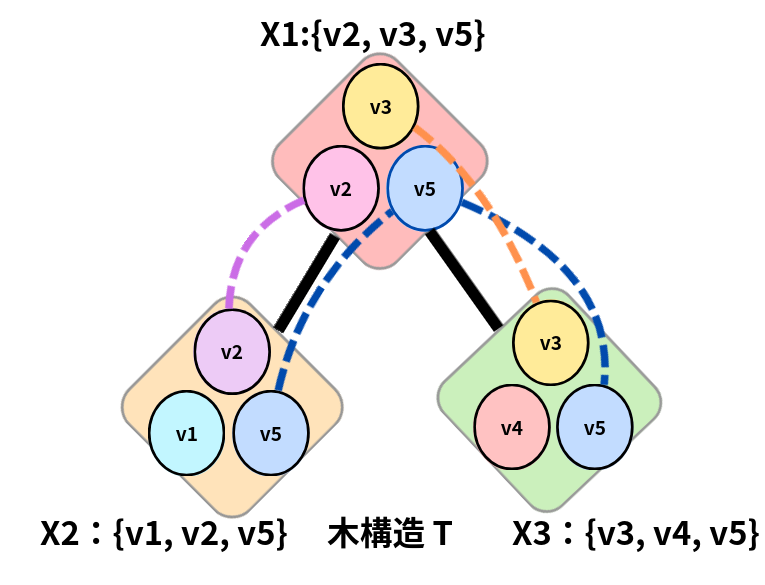
\includegraphics[width=0.35\textwidth]{tree-decomposition-rule.png}
  \caption{木分解の例}
\end{figure}

\FloatBarrier
\subsection{木幅の計算}

与えられたグラフ$G$の木幅が求められれば，動的計画法や分割統治法を適用して問題を高速に解くことができる.
しかし，木幅を求めるには木分解を行うこととなり，これを高速に得られることが重要である.
木分解のアルゴリズムの詳細は文献\cite{bodlaender2010treewidth}を参照されたい.
ここでは，原理を学ぶために率直な方法のみ紹介する.

\subsubsection{消去順序（Elimination Ordering）}
グラフ $G=(V, E)$ の木幅 $tw(G)$ を求める問題は，
頂点集合 $V$ のある順列 $\pi = (v_1, v_2, \dots, v_n)$ を見つけ，
その順序で頂点を消去（Elimination）した際に発生するフィルイン（追加エッジ）を含めたグラフ $G^*$ を
弦グラフ（Chordal Graph）にすることと同値である．
このとき，木幅は $G^*$ の最大クリークサイズ − 1 で表される.

\subsubsection{アルゴリズム}
全ての可能な消去順序の集合 $\Pi = \{\pi_1, \pi_2, \dots, \pi_{n!}\}$ を走査し，
各順序における幅を計算する．

\begin{enumerate}
    \item \textbf{順列の生成}\\ 頂点集合 $V$ のすべての置換 $\pi \in \Pi$ を列挙する.

    \item \textbf{消去プロセスの実行}\\
    各順序 $\pi$ に従い, 各頂点 $v_i$ に対して $i=1$ から $n$ まで以下を行う.
    \begin{enumerate}
        \item $v_i$ の隣接頂点集合を $N(v_i)$ とする,
        \item $N(v_i)$ 内の互いに隣接していない頂点をすべて結び, 完全グラフ（クリーク）にする（フィルイン）,
        \item $v_i$ のバッグ $X_{v_i} = \{v_i\} \cup \{v_j \in N(v_i) \mid \pi(v_j) > \pi(v_i)\}$ を作る, 
        \item このバッグのサイズ − 1 を, そのステップでの幅として記録する,
        \item $v_i$ を取り除く
    \end{enumerate}

    \item \textbf{順序 $\pi$ における幅の決定}\\
    順列 $\pi$ における幅 $w(\pi)$ を，各ステップで記録した次数の最大値として算出する. 
    \[
    w(\pi) = \max_{1 \le i \le n} (|X_{v_i}| - 1)
    \]

    \item \textbf{木幅の決定}\\
    すべての順列の中で $w(\pi)$ を最小にする値を木幅 $tw(G)$ とする.
    \[
    tw(G) = \min_{\pi \in \Pi} w(\pi)
    \]
\end{enumerate}

[例1]
図\ref{Elimination}において順序(A, B, C, D)の場合の消去順序は以下の通りとなる.
\begin{enumerate}
  \item 頂点Aの隣接頂点集合$\{A, B, D\}$を作り, バッグ$X_1$とする. B, Dは辺で結ばれていないため辺で結び, 頂点Aを削除する
  \item 頂点Bの隣接頂点集合$\{B, C, D\}$を作り, バッグ$X_2$とする. 頂点Bを削除する
  \item 頂点Cの隣接頂点集合$\{C, D\}$を作り, バッグ$X_3$とする. 頂点Cを削除する
  \item 頂点Dの隣接頂点集合$\{D\}$を作り, バッグ$X_4$とする. 頂点Dを削除する
  \item したがって, 木幅は$3-1=2$となる
\end{enumerate}

消去順序を用いた場合, 各ステップのバッグをその中の頂点が次に現れるバッグへ結ぶと必ず木になるため木分解は\ref{elimitnate-tree}のようになる. 
\begin{figure}[h]
  \centering
  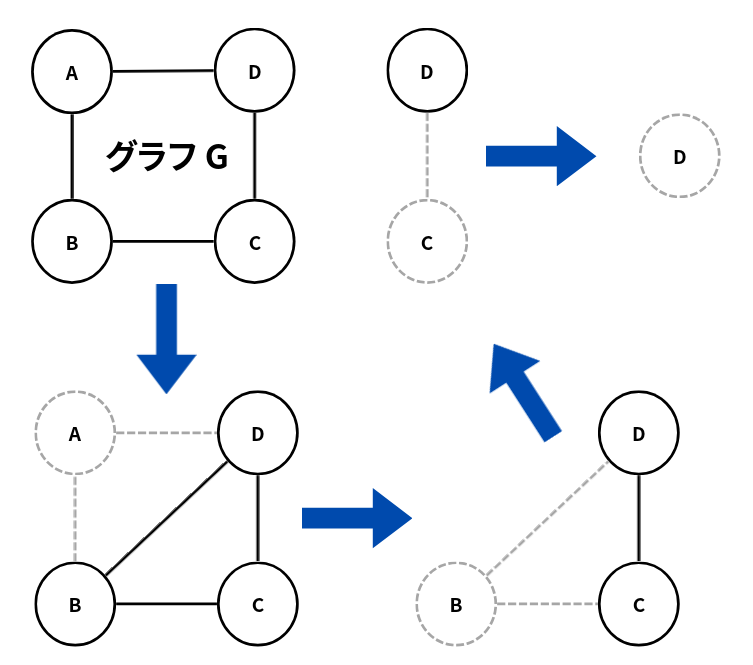
\includegraphics[width=0.4\textwidth]{example1.png}
  \caption{順序削除の例}
  \label{Elimination}
\end{figure}  

\begin{figure}[h]
  \centering
  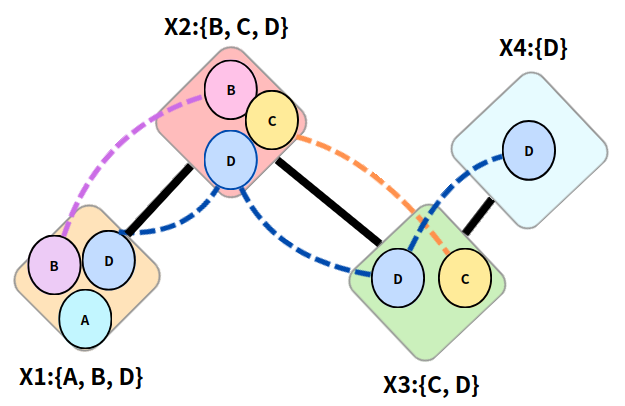
\includegraphics[width=0.4\textwidth]{eliminate-tree.png}
  \caption{\ref{Elimination}を木分解して得られた木T}
  \label{elimitnate-tree}
\end{figure}  

木分解の最小幅を求める問題はNP困難であるため, 実用的な時間である程度良い解を得る近似アルゴリズムとして
貪欲法や次数に基づく対数近似, 平面グラフに対する近似, セパレータ法などがある\cite{bodlaender2010treewidth}.


\section{学習支援システムの設計}

本研究では，木幅および木分解の定義理解を目的として，
問題演習を通じて学習を支援するシステムを設計・実装する．
本システムは，木分解に関する定義や性質を段階的に確認できる
問題形式を採用することで，学習者の理解を促進することを目的とする．

\subsection{設計方針}
木幅および木分解の理解には，定義を正確に把握し，
それを具体的なグラフ構造に適用する力が求められる．
しかし，従来の学習では定義を読んだだけでは理解が定着しにくいという課題がある．

そこで本システムでは，以下の方針に基づいて設計を行った．
\begin{itemize}
  \item 木分解の定義や性質を，問題形式で確認できるようにする,
  \item 様々な問題形式を用いて，理解度を即時に確認できるようにする, 
  \item 問題は段階的に難易度を上げ，定義理解から応用へと導く構成とする, 
  \item 画面上でグラフの頂点や辺をクリックでインタラクティブに選択できるようにする
\end{itemize}

本システムは，学習者に最初から木分解の構築を求めるのではなく，
定義理解を確認する問題演習を通じて，
学習者が必要な前提知識を段階的に獲得できる点に特徴がある．
また, 学習者がインタラクティブにグラフや木構造に触れられるようにするためには
グラフや木構造の頂点や辺の情報を保持しておく必要がある. 
したがって，問題作成時には画像を挿入するのではなく，ツールを利用してグラフを生成できるようにしている.

\subsection{問題形式の構成}
本システムでは，主に以下の問題形式を実装している．

\subsubsection{○×問題}
○×問題では，木分解や木幅に関する命題などを提示し，
学習者がその正誤を選択する．
これにより，定義の誤解や曖昧な理解を顕在化させることができる．

例として，「あるグラフの木幅が1であるとき，そのグラフは必ず木である」
といった命題を扱う．

\subsubsection{入力問題}
入力問題では，学習者が数値や簡単な記号を入力することで解答を行う．
例えば，提示されたグラフに対して，
その木幅や特定の木分解における幅を求めさせる問題を用意している．
この形式により，単なる選択ではなく，
定義に基づいた計算や判断を要求することができる．

\subsubsection{選択問題}
選択問題では，複数の選択肢の中から正しいものを選ばせることで，
木分解や木幅に関する理解を確認する．
この形式は，単純な正誤判定よりも多様な誤答パターンを提示できるため，
学習者が自身の誤解の内容を把握しやすいという利点がある．

例えば，木分解の条件（TD1--TD3）に関する説明のうち，
正しいものを選択させる問題や，
提示された木分解が正しいかどうかを選択肢から判断させる問題を扱っている．

\subsection{使用技術}
本Webシステムの実装には，表\ref{tab:tech}に示す技術を用いた. 
以下に，各技術の選定理由を述べる.
\begin{table}[h]
  \centering
  \caption{本Webシステムで使用した技術}
  \label{tab:tech}
  \begin{tabular}{ll}
    \hline
    区分 & 使用技術 \\ \hline
    実行環境 & Node.js \\
    プログラミング言語 & TypeScript \\
    フレームワーク & Next.js \\
    UI ライブラリ & React \\
    データベース & SQLite \\
    ORM & Prisma \\
    グラフ描画ライブラリ & ReactFlow \\
    \hline
  \end{tabular}
\end{table}

Node.js\cite{nodejs} は，JavaScript言語を用いてサーバー側の処理を実行できる環境である．
非同期処理を効率よく行える点から採用した．
また，フロントエンド（ブラウザで動く部分）と同じ言語でサーバー処理を書けるため，開発が容易である．
Next.js\cite{Next.js} と組み合わせることで，ページ遷移やデータ管理の実装が簡単になり，Webアプリケーション全体の構築効率が向上する．

TypeScript\cite{TypeScript} は，JavaScriptに型付けの機能を追加した言語である．
型付けによってプログラムのミスを防ぎやすくなり，複雑なデータ構造を扱う本システムにおいて安全性と保守性を向上させる．

Next.jsはReact\cite{React,React/Next.js,React2025,Webprogramming}を基盤としたWebフレームワークであり，Webページの構築や状態管理を容易にする．
本研究では，学習者がグラフ構造を操作する画面を構築する際に便利であるため採用した．

React はコンポーネント指向のユーザインタフェース（UI）ライブラリであり，
画面の状態変化に応じて動的に表示を更新できる．
これにより，学習者が操作した結果をリアルタイムに画面へ反映できる．

SQLite\cite{sqlite} は軽量な組込み型データベースであり，追加のデータベースサーバを必要としない．
本研究では小規模なデータ管理を想定しており，SQLiteで十分な性能を得られる．

Prisma\cite{Prisma} はTypeScriptと親和性の高いORM（データベース操作をコードで簡単に行える仕組み）である．
これにより，データベースのスキーマとアプリケーションコード間の不整合を防ぎつつ，安全にデータ操作を行える．

ReactFlow\cite{reactflow} は，ノードとエッジからなるグラフ構造を直感的に描画・操作できるライブラリである．
本研究では，木分解や木幅の学習支援を目的として学習者がグラフを動的に編集・確認できる点で有用である．

\subsection{実装状況}
本システムでは，現時点で以下の機能を実装している．
\begin{itemize}
  \item 問題提示（○×・入力・選択問題）,
  \item 解答・正誤判定,
  \item 問題ごとの解説表示,
  \item インタラクティブなグラフを含めた問題追加
\end{itemize}

図\ref{TrueOrFalse}に○×問題の問題提示画面の例を示す．
ここでは，グラフGを示しその木幅が1であるかどうかを問いている．
木幅が1であるグラフは木構造であるので，答えは×である．

また，図\ref{Input}に入力問題の問題提示画面の例を示す．
ここでは，条件2を満たすために足りない辺の数を問いている．
この場合，辺を構成する頂点$(u,w)$のうち$(v6,v9)$が同じバッグに属していない．
したがって，答えは1となる．

同様に，図\ref{Choice}に選択問題の問題提示画面の例を示す．
ここでは，提示したバッグの割り当てが条件1を満たしているかどうかを問いている．
この場合，「どのバッグも$v7$が属していないため，条件1は満たされていない．」が解となる．


\section{今後の課題}
今後の課題を以下に示す．
\begin{itemize}
  \item 問題を自動で生成する機能の追加,
  \item 様々なグラフを自動で生成する機能,
  \item 様々な木分解アルゴリズムの実装とそれらを適用した結果をグラフィカルに表示する機能,
  \item 学習者の解答履歴を用いた理解度分析
\end{itemize}
これらは現在，順次，実装を予定している．
一方で，一般の大学生にこれを勉強したいかと質問したところ，「無味乾燥である」との感想が残念ながらあった．
そこで，ゲームをしながら木分解を学べないかを検討したい．


\section{まとめ}
木幅と木分解の定義理解を目的としたWebアプリケーションによる学習システムを構築した．
Webアプリケーションの主要技術にはアプリケーションの開発容易性やプログラムミスなどを防ぐため，
そして，インタラクティブなシステムとするために，Node.js，Next.js，React，Typescript，SQLite，Prisma，そしてReactFlowなどの技術を活用した．
\ack %% 謝辞
\noindent 本研究の一部は，日本学術振興会科学研究費助成事業（基盤研究(A)）課題番号JP24H00697の助成による．
\bibliographystyle{unsrt}
\bibliography{refs}

\begin{figure}[b]
  
\includegraphics[width=0.58\textwidth]{TrueOrFalse.png}  
  \caption{○×問題の例}
  \label{TrueOrFalse}
\end{figure}
\begin{figure}[p]
  
\includegraphics[width=0.58\textwidth]{Input.png}  
  \caption{入力問題の例}
  \label{Input}
\end{figure}
\begin{figure}[p]
  
\includegraphics[width=0.58\textwidth]{Choice.png}  
  \caption{選択問題の例}
  \label{Choice}
\end{figure}


%\appendix
%\section{}
 
%% 著者紹介・顔写真の掲載はC分冊の場合は任意です．
\begin{biography}
\profile{}{}{}
%\profile{会員種別}{名前}{紹介文}% 顔写真あり
%\profile*{会員種別}{名前}{紹介文}% 顔写真なし
\end{biography}

\end{document}



